\documentclass[10pt,xcolor={dvipsnames}]{beamer}
% Class options include: notes, notesonly, handout, trans,
%                        hidesubsections, shadesubsections,
%                        inrow, blue, red, grey, brown

% Theme for beamer presentation.
%\usepackage{beamerthemelined} 
%\usepackage{times}
%\usepackage[usenames,dvipsnames]{xcolor}
\usepackage{anysize}
\usepackage{fancyhdr}
\usepackage{graphicx}
\usepackage{pdfpages}
\usepackage{amsmath}
\usepackage{tikz}
\usepackage{amssymb}
\usepackage{caption}
\usepackage{listings}
\usepackage{multirow}
\usepackage{hyperref}
 \hypersetup{
 colorlinks=true,
 linkcolor=black
 }
% Other themes include: beamerthemebars, beamerthemelined, 
%                       beamerthemetree, beamerthemetreebars  

\title{\bfseries Term Indexing for the \\ Beagle Theorem Prover}    % Enter your title between curly braces
\author{Tim Cosgrove \vspace{-0.3cm}}                 % Enter your name between curly braces
\institute{COMP4006 Honours Research Project \\ \vspace{0.3cm}
Research School of Computer Science,\\
Australian National University \\ \vspace{0.3cm}
\texttt{u4843619@anu.edu.au} \\ \vspace{0.3cm}
Supervisor: Peter Baumgartner}      % Enter your institute name between curly braces
\date{\today}                    % Enter the date or \today between curly braces

\usetheme{Hannover}
\usecolortheme{orchid}
\setbeamertemplate{navigation symbols}{}

\newcommand{\bcen}{\begin{center}}
\newcommand{\ecen}{\end{center}}
\newcommand{\HSWAC}{Hierarchic Superposition with Weak Abstraction Calculus}
\newcommand{\HSWA}{Hierarchic Superposition with Weak Abstraction}
\newcommand{\compY}{\textcolor{Green}{\textbf{Y}}}
\newcommand{\compN}{\textcolor{Red}{\textbf{N}}}
\newcommand{\tcent}[1] {\vspace{-0.7cm}\begin{center}
#1
\end{center}\vspace{-0.1cm}}
\newcommand{\cent}[1] {\begin{center}
#1
\end{center}}

\begin{document}

\begin{NoHyper}
% Creates title page of slide show using above information
\begin{frame}
  \titlepage
\end{frame}
\note{} % Add notes to yourself that will be displayed when
        % typeset with the notes or notesonly class options

\section[Outline]{}

% Creates table of contents slide incorporating
% all \section and \subsection commands
\begin{frame}
  \tableofcontents
\end{frame}
%%%%%%%%%%%%%%%%%%%%%%%%%%%%%%%%%%%%%%%%%%%%%%%%%%%%%%%%%%%%%%%%%%%%%%%%%%%%%%%%
\section{Project Overview}
%%%%%%%%%%%%%%%%%%%%%%%%%%%%%%%%%%%%%%%%%%%%%%%%%%%%%%%%%%%%%%%%%%%%%%%%%%%%%%%%

\subsection{Motivation}

\begin{frame}
  \frametitle{The Beagle Theorem Prover}
  \begin{itemize}
  \item<1-> Beagle is a First-Order-Logic resolution theorem prover with equality,
            built to show off the capabilities of the \HSWAC.
  \item<2-> This calculus is capable of \emph{hierarchic reasoning} by incorporating a
  \emph{background prover}.
  \item<2-> Background provers act as a black box which can instantly prove
  known facts. For example integer arithmetic.
  \item<3-> The calculus is carefully constructed with a process known as
  \emph{weak abstraction} in order to ensure consistency and completeness.
  \end{itemize}
\end{frame}

{
\usebackgroundtemplate{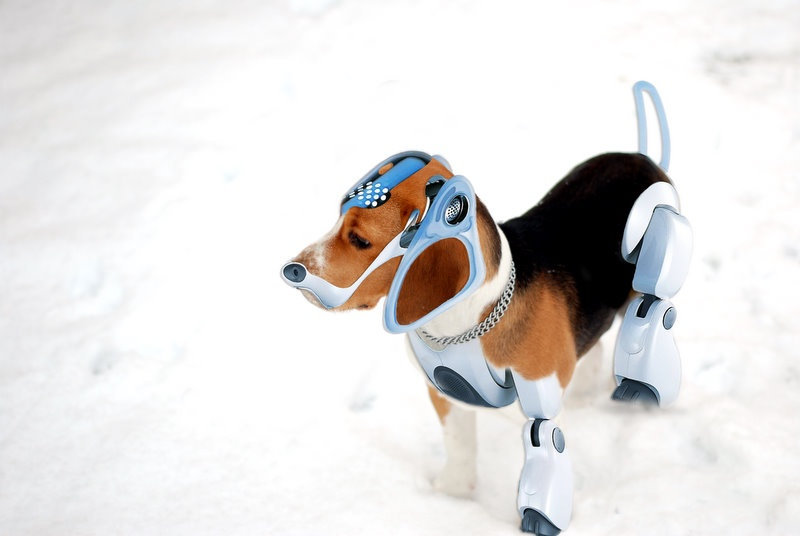
\includegraphics[width=\paperwidth]{robobeagle}}
\begin{frame}
  \frametitle{Extending Beagle}
  \begin{itemize}
  \item<1-> Beagle has some major shortcomings which prevent it being more than
  a proof of concept.
  \item<1-> In particular, it lacks an efficient manner of locating terms for inference.
  \item<2-> Enter 'Term Indexing', a method for efficiently managing and collecting
  these terms.
  \item<3-> Research Questions:
    \begin{itemize}
    \item<3-> How can Term Indexing (in particular Fingerprint Indexing) be implemented
    and applied to Beagle?
    \item<3-> How can Fingerprint Indexing be improved; generally and with respect to
    Beagle's specific calculus?
    \item<3-> What sort of improvement will this implementation yield in the prover?
    \end{itemize}
  \end{itemize}
\end{frame}
}

%%%%%%%%%%%%%%%%%%%%%%%%%%%%%%%%%%%%%%%%%%%%%%%%%%%%%%%%%%%%%%%%%%%%%%%%%%%%%%%%
\section{Background}
%%%%%%%%%%%%%%%%%%%%%%%%%%%%%%%%%%%%%%%%%%%%%%%%%%%%%%%%%%%%%%%%%%%%%%%%%%%%%%%%

%%%%%%%%%%%%%%%%%%%%%%%%%%
\subsection{First Order Logic Terminology}
%%%%%%%%%%%%%%%%%%%%%%%%%%

\begin{frame}
  \frametitle{Terminology Used in this Presentation}
  \begin{itemize}
  \item<1-> First Order Logic
  \item<2-> Positions
  \item<3-> Substitutions:
    \begin{itemize}
    \item<3-> $s$ is '\emph{unifiable}' with $t$ : $\sigma s = \sigma t$
    \item<3-> $s$ '\emph{subsumes}' $t$ : $\sigma s = t$
    \end{itemize}
  \end{itemize}
\end{frame}

%%%%%%%%%%%%%%%%%%%%%%%%%%
\subsection{The Beagle Theorem Prover}
%%%%%%%%%%%%%%%%%%%%%%%%%%

\begin{frame}
  \frametitle{The Superposition Calculus}
  \begin{itemize}
  \item<1-> Normal Superposition rule
  \end{itemize}
  \begin{align*}
&\textbf{Positive Superposition}\ \ \ \ \  \frac{l \approx r \lor C\quad \quad s[u] \approx t \lor D}{(s[r] \approx t \lor C \lor D)\sigma}\\
\text{Where } &(i) \text{ $\sigma = $ simple mgu $(l,u)$,}\\
\text{and } &(ii) \text{ $u$ is not a variable.}
\end{align*}
\end{frame}

\begin{frame}
  \frametitle{The \HSWAC}
  \begin{itemize}
  \item<1-> Extension of the Superposition Calculus to accommodate hierarchic reasoning.
  \end{itemize}
  \begin{align*}
&\textbf{Positive Superposition}\ \ \ \ \  \frac{l \approx r \lor C\quad \quad s[u] \approx t \lor D}{\text{abstr}((s[r] \approx t \lor C \lor D)\sigma)}\\
\text{Where } &(i) \text{ $\sigma = $ simple mgu $(l,u)$,}\\
&(ii) \text{ $u$ is not a variable,}\\
&(iii) \text{ $r\sigma \not\succeq l\sigma$,}\\
&(iv) \text{ $t\sigma \not\succeq s\sigma$,}\\
&(v) \text{ $l$ and $u$ are not pure background terms,}\\
&(vi) \text{ $(l \approx r)\sigma$ is strictly maximal in $(l \approx r \lor C)\sigma$,}\\
\text{and } &(vii) \text{ $(s \approx t)\sigma$ is strictly maximal in $(s \approx t \lor D)\sigma$.}
\end{align*}
\end{frame}

%%%%%%%%%%%%%%%%%%%%%%%%%%
\subsection{Term Indexing} 
%%%%%%%%%%%%%%%%%%%%%%%%%%
\begin{frame}
  \frametitle{Term Indexing Techniques}
  \begin{itemize}
  \item<1-> Term indexers aim to collect all FOL terms which potentially match a `query' term.
  \item<2-> Top-Symbol Hashing.
  \item<2-> Discrimination Trees.
  \item<2-> Path Indexing.
  \end{itemize}
\end{frame}

%%%%%%%%%%%%%%%%%%%%%%%%%%
\subsection{Fingerprint Indexing} 
%%%%%%%%%%%%%%%%%%%%%%%%%%
\begin{frame}
  \frametitle{Fingerprint Indexing}
                  %Left Bot Right Top
  \begin{itemize}
  \item<1-> Maintain a collection of \emph{fingerprints} for terms.
  \item<2-> A term fingerprint is an array over $F \cup \{\mathbf{A, B, N}\}$,\\ the \emph{Fingerprint Features.}
  \item<3->[] 
  {\small \begin{table}\caption{Fingerprint Feature comparison tables for \emph{unification}
  (left) and \emph{subsumption} (right)}\begin{tabular}{| c || c | c | c | c | c |}
  \hline
           &  $f_1$      &  $f_2$      &  \textbf{A} &  \textbf{B} &  \textbf{N} \\ \hline \hline
  $f_1$    &  \compY &  \compN &  \compY &  \compY &  \compN \\ 
  $f_2$    &  \compN &  \compY &  \compY &  \compY &  \compN \\ 
\textbf{A} &  \compY &  \compY &  \compY &  \compY &  \compN \\
\textbf{B} &  \compY &  \compY &  \compY &  \compY &  \compY \\ 
\textbf{N} &  \compN &  \compN &  \compN &  \compY &  \compY \\ \hline
  \end{tabular}\ \ \ \ \ \ \begin{tabular}{| c || c | c | c | c | c |}
  \hline
           &  $f_1$      &  $f_2$      &  \textbf{A} &  \textbf{B} &  \textbf{N} \\ \hline \hline
  $f_1$    &  \compY &  \compN &  \compN &  \compN &  \compN \\ 
  $f_2$    &  \compN &  \compY &  \compN &  \compN &  \compN \\ 
\textbf{A} &  \compY &  \compY &  \compY &  \compN &  \compN \\
\textbf{B} &  \compY &  \compY &  \compY &  \compY &  \compY \\ 
\textbf{N} &  \compN &  \compN &  \compN &  \compN &  \compY \\ \hline
  \end{tabular}\end{table}}\vspace{0.5cm}
  \item<4-> {\footnotesize Schulz, Stephan: Fingerprint Indexing for Paramodulation and Rewriting. In:
  Lecture Notes in Computer Science volume 7364 pp. 447--483 (2012).}

  \end{itemize}
\end{frame}

%  \begin{frame}
%  \frametitle{Fingerprint Indexing -- Potential Performance}
%  \begin{center}{\tiny
%  \begin{tabular}{| l | r | r | r | r | r | r | r |} \hline
%  Index & Run time & Sat time & PM time & PMI time & MGU time & BR time & BRI time \\ \hline
%NoIdx & 16062.392 & 14078.300 &  8980.320 & 0.000 & 2545.080  & 2280.250 & 0.000\\
%FP1 & 7006.758 & 6145.870 & 1816.100 & 25.710 & 450.760 & 379.570 & 40.150\\
%FP6M & 6000.177 & 5385.810 & 1181.710 & 38.240 & 99.110 & 39.010 & 55.660\\
%NPDT & 6082.246 & 5434.760 & 1184.750 & 64.910 & 83.110 & 33.200 & 79.910 \\\hline
%  \end{tabular}}\vspace{0.5cm}
%                  %Left Bot Right Top
%  \includegraphics[page=13,scale=0.5,trim=6cm 8cm 7cm 12cm,clip]{schulz_fp-index_ext}
%  \hspace{1cm}
%                  %Left Bot Right Top
%  \includegraphics[page=14,scale=0.5,trim=6cm 16.2cm 7cm 4cm,clip]{schulz_fp-index_ext}
%  \end{center}
%\end{frame}

\begin{frame}
  \frametitle{Fingerprint Indexing -- Example Fingerprint Index}
                  %Left Bot Right Top
  \includegraphics[page=7,scale=0.7,trim=4cm 13.5cm 5cm 4.5cm,clip]{schulz_fp-index_ext}
\end{frame}

\begin{frame}
  \frametitle{Why Fingerprint Indexing?}
  \begin{itemize}
  \item<1-> New and not thoroughly tested technique.
  \item<2-> Currently showing very promising results.
  \item<3-> Highly customisable and configurable.
  \end{itemize}
\end{frame}

%%%%%%%%%%%%%%%%%%%%%%%%%%%%%%%%%%%%%%%%%%%%%%%%%%%%%%%%%%%%%%%%%%%%%%%%%%%%%%%%
\section{Implementation}
%%%%%%%%%%%%%%%%%%%%%%%%%%%%%%%%%%%%%%%%%%%%%%%%%%%%%%%%%%%%%%%%%%%%%%%%%%%%%%%%

%%%%%%%%%%%%%%%%%%%%%%%%%%
\subsection{Implementing Fingerprint Indexing}
%%%%%%%%%%%%%%%%%%%%%%%%%%
\begin{frame}
  \frametitle{Creating the Fingerprint Index}
  \begin{itemize}
  \item<1-> Addition of terms.
  \item<2-> Requires an Fingerprint generation along with implementation and traversal of the Index tree structure.
  \item<3-> Retrieval of terms.
  \item<4-> Requires implementation of the comparison tables and a more complex
  Index traversal algorithm.
  \end{itemize}
\end{frame}

%%%%%%%%%%%%%%%%%%%%%%%%%%
\subsection{Indexing Applications}
%%%%%%%%%%%%%%%%%%%%%%%%%%
\begin{frame}
  \frametitle{Beagle's Main Procedure}
  \begin{itemize}
  \item<1-> 
Maintain two Clause Sets, \emph{new} and \emph{old}.\\
Remove Clauses from \emph{new} one at a time, simplify them and then
attempt inference rules.
  \item<2-> Two key areas of improvement ($O(n)$ operations):
  \begin{itemize}
  \item<2-> Inferences via the Superposition rules.
  \item<2-> Simplifying Clauses.
  \end{itemize}
  \end{itemize}
\end{frame}

\begin{frame}
  \frametitle{Indexing Superposition}
  \begin{itemize}
  \item<1->[]
  \begin{align*}
&\textbf{Positive Superposition}\ \ \ \ \  \frac{l \approx r \lor C\quad \quad s[u] \approx t \lor D}{\text{abstr}((s[r] \approx t \lor C \lor D)\sigma)}\\
\text{Where } &(i) \text{ $\sigma = $ simple mgu $(l,u)$,}\\
&(ii) \text{ $u$ is not a variable,}\\
&(iii) \text{ $r\sigma \not\succeq l\sigma$,}\\
&(iv) \text{ $t\sigma \not\succeq s\sigma$,}\\
&(v) \text{ $l$ and $u$ are not pure background terms,}\\
&(vi) \text{ $(l \approx r)\sigma$ is strictly maximal in $(l \approx r \lor C)\sigma$,}\\
\text{and } &(vii) \text{ $(s \approx t)\sigma$ is strictly maximal in $(s \approx t \lor D)\sigma$.}
\end{align*}
  \item<1-> Requires that we index all subterms. Furthermore we must implement two
  separate cases for \emph{from} and \emph{into}.

  \end{itemize}
\end{frame}

\begin{frame}
  \frametitle{Indexing Simplification}
  \begin{itemize}
  \item<1-> Simplification rules exist to implement special cases of the rules
  in the \HSWAC.
  \item<1-> These special cases allow redundant Clauses to be removed; preventing
  clutter in the inference process.
  \item<2-> The two main simplification rules used by Beagle are \emph{Negative Unit Simplification}
  and \emph{Demodulation}
  \item<3-> These rules operate only on \emph{unit Clauses}, so using our current
  index clogged with subterms is inefficient.
  \item<3-> The rules also require checking for \emph{subsumption}, which requires 
  implementing a new comparison table for Fingerprint Indexing.
  \end{itemize}
\end{frame}

\begin{frame}
  \frametitle{Indexing Negative Unit Simplification}
  \begin{itemize}
  \item<1->[] 
\begin{align*}
&\textbf{Negative Unit Simplification}\ \ \ \ \ \frac{l\not\approx r \quad \quad s \approx t  \lor C}{C}\\
&\text{Where } (i)\ \  \exists \sigma\ \  s.t.\ \  (l \approx r)\sigma \equiv s \approx t.\\
&\text{The clause $s \approx t  \lor C$ may be removed.}
\end{align*}
  \item<2-> Searching for valid subsuming Literals is extremely time consuming.
  \item<2-> Requires an index capable of matching Equations rather than Terms.
  \end{itemize}
\end{frame}

\begin{frame}
  \frametitle{Indexing Demodulation}
  \begin{itemize}
  \item<1->[] 
\begin{align*}
&\textbf{Demodulation}\ \ \ \ \ \frac{l \to r \quad \quad s[u] \approx t  \lor D}{ s[r\sigma] \approx t \lor D}\\
&\text{Where } l\sigma = u\\
&\text{The clause $s[u] \approx t  \lor D$ may be removed.}
\end{align*}
  \item<2-> For a simple example, with a Literal $X \to f(a)$ we may replace all occurrences of $X$ with $f(a)$.
  \item<3-> Like in Negative Unit Simplification, the most costly operation is searching
  for subsuming $l$ Terms.
  \item<3-> We must perform this search for every possible subterm $u$ of $s$.
  \end{itemize}
\end{frame}

%%%%%%%%%%%%%%%%%%%%%%%%%%
\subsection{Tailoring to Beagle}
%%%%%%%%%%%%%%%%%%%%%%%%%%
\begin{frame}
  \frametitle{Fingerprint Indexing for the Hierarchic Superposition with Weak Abstraction Calculus}
                  %Left Bot Right Top
  \begin{itemize}
  \item<1-> The \HSWAC\ imposes many restrictions on what can be used for inference.
  \item<2-> We may take advantage of some of these conditions to increase the effectiveness of Fingerprint Indexing.
  \item<3->[]\begin{table}[H]\scriptsize
  \caption{Fingerprint comparison table for unification; extended by considering the term hierarchy.}
  \label{tab:extunif}
  \begin{tabular}{| c || c | c | c | c | c || c | c | c | c |}
  \hline
            &  $f_1$  &  $f_2$  &  \textbf{A} &  \textbf{B} &  \textbf{N} &    $f_1$+  & $f_2$+  & \textbf{A}+ & \textbf{B}+ \\ \hline \hline
  $f_1$     &  \compY &  \compN &  \compY     &  \compY     &  \compN     &    \compN  & \compN  & \compN      & \compN      \\ 
  $f_2$     &  \compN &  \compY &  \compY     &  \compY     &  \compN     &    \compN  & \compN  & \compN      & \compN      \\ 
\textbf{A}  &  \compY &  \compY &  \compY     &  \compY     &  \compN     &    \compY  & \compY  & \compY      & \compY      \\
\textbf{B}  &  \compY &  \compY &  \compY     &  \compY     &  \compY     &    \compY  & \compY  & \compY      & \compY      \\ 
\textbf{N}  &  \compN &  \compN &  \compN     &  \compY     &  \compY     &    \compN  & \compN  & \compN      & \compY      \\ \hline \hline
%
$f_1$+      &  \compN &  \compN &  \compY     &  \compY     &  \compN     &    \compY  & \compN  & \compY      & \compY      \\ 
$f_2$+      &  \compN &  \compN &  \compY     &  \compY     &  \compN     &    \compN  & \compY  & \compY      & \compY      \\ 
\textbf{A}+ &  \compN &  \compN &  \compY     &  \compY     &  \compN     &    \compY  & \compY  & \compY      & \compY      \\
\textbf{B}+ &  \compN &  \compN &  \compY     &  \compY     &  \compY     &    \compY  & \compY  & \compY      & \compY      \\ \hline
  \end{tabular}\end{table}
  \end{itemize}

\end{frame}


%%%%%%%%%%%%%%%%%%%%%%%%%%%%%%%%%%%%%%%%%%%%%%%%%%%%%%%%%%%%%%%%%%%%%%%%%%%%%%%%
\section{Results}
%%%%%%%%%%%%%%%%%%%%%%%%%%%%%%%%%%%%%%%%%%%%%%%%%%%%%%%%%%%%%%%%%%%%%%%%%%%%%%%%

%%%%%%%%%%%%%%%%%%%%%%%%%%
\subsection{Evaluation Metrics}
%%%%%%%%%%%%%%%%%%%%%%%%%%
\begin{frame}
  \begin{itemize}
  \frametitle{Metrics for Analysing Indexing Performance}
  \item<1-> Total run time - Need to be careful to consider all factors.
  \item<2-> False Positives - Relevant, but can be misleading depending on
  number of positions being sampled.
  \item<3-> Run time \emph{per Inference} - Most accurate measure of performance.
  Must still take care when interpreting.
  \end{itemize}
\end{frame}


%%%%%%%%%%%%%%%%%%%%%%%%%%
\subsection{Beagle Comparisons}
%%%%%%%%%%%%%%%%%%%%%%%%%%

\begin{frame}
  \frametitle{Comparing Varieties of Beagle}
  \begin{table}[H]\scriptsize
  \caption{Totalled inference counts and indexing statistics for various versions of beagle.}
\begin{tabular}{| l || r | r | r || r | r | r |}  \cline{2-7}
\multicolumn{1}{ c }{} & \multicolumn{3}{ |c|| }{\textbf{Inference Counts}} & \multicolumn{3}{ c| }{\textbf{Indexing Results}} \\ \cline{1-7}
Version&Sup&Demod&NegUnit&TotalFound&SupFP&SimpFP\\  \cline{1-7}
\textbf{Unmodified \footnotemark[1]}&414216&29097&1826&0&0&0\\
\textbf{Standard}&162881&41414&2452&61884768&15525&39778148\\
\textbf{Enhanced}&146861&35326&1960&58119897&17641&39916687\\  \hline
\end{tabular}\end{table}
\begin{table}[H]\scriptsize
  \caption{Totalled timing results for various versions of beagle.}
\begin{tabular}{| l || r | r | r | r | r | r |}  \cline{2-7}
\multicolumn{1}{ c }{} & \multicolumn{6}{| c| }{\textbf{Time Spent (seconds)}} \\ \cline{1-7}
Version&Indexing&Retrieving&Sup&Demod&NegUnit&Total\\  \cline{1-7}
\textbf{Unmodified \footnotemark[1]}&0&0&730.44&9.44&31.99&5623.21\\
\textbf{Standard}&28.4&38.73&254.17&41.66&3.18&381.36\\
\textbf{Enhanced}&18.74&17.58&168.79&30.56&2.12&259.02\\ \hline
\end{tabular}\end{table}


\footnotetext[1]{{\footnotesize This version failed to solve two out of the fifty problems within 8 hours.}}
\end{frame}

\begin{frame}
  \begin{itemize}
  \frametitle{Results Analysis}
  \item<1->[]
  \frametitle{Time Spent Per Inference}
 \begin{table}[H]\scriptsize
  \caption{Superposition time for the 6 most extreme problem examples.}
\begin{tabular}{| l || r | r | r |}  \hline
Version&Superposition&Demodulation&NegUnit Simplification\\  \hline
\textbf{Unmodified}&1.7ms & 0.3ms & 17.5ms  \\
\textbf{Standard}  &1.5ms & 1.0ms & 1.3ms  \\
\textbf{Enhanced}  &1.1ms & 0.8ms & 1.0ms  \\\hline
\end{tabular}\end{table}  
\item<2-> Most typical application of Demodulation is a Literal like $X \to f(a)$.
$X$ will match anything, making fingerprint indexing a waste of time.
\item<3-> When excluding PUZ037-1.p we have 0.29, 0.39 and 0.31 milliseconds per Demodulation.
  \end{itemize}
\end{frame}



\begin{frame}
  \frametitle{Runtimes under 5 seconds}
                  %Left Bot Right Top
  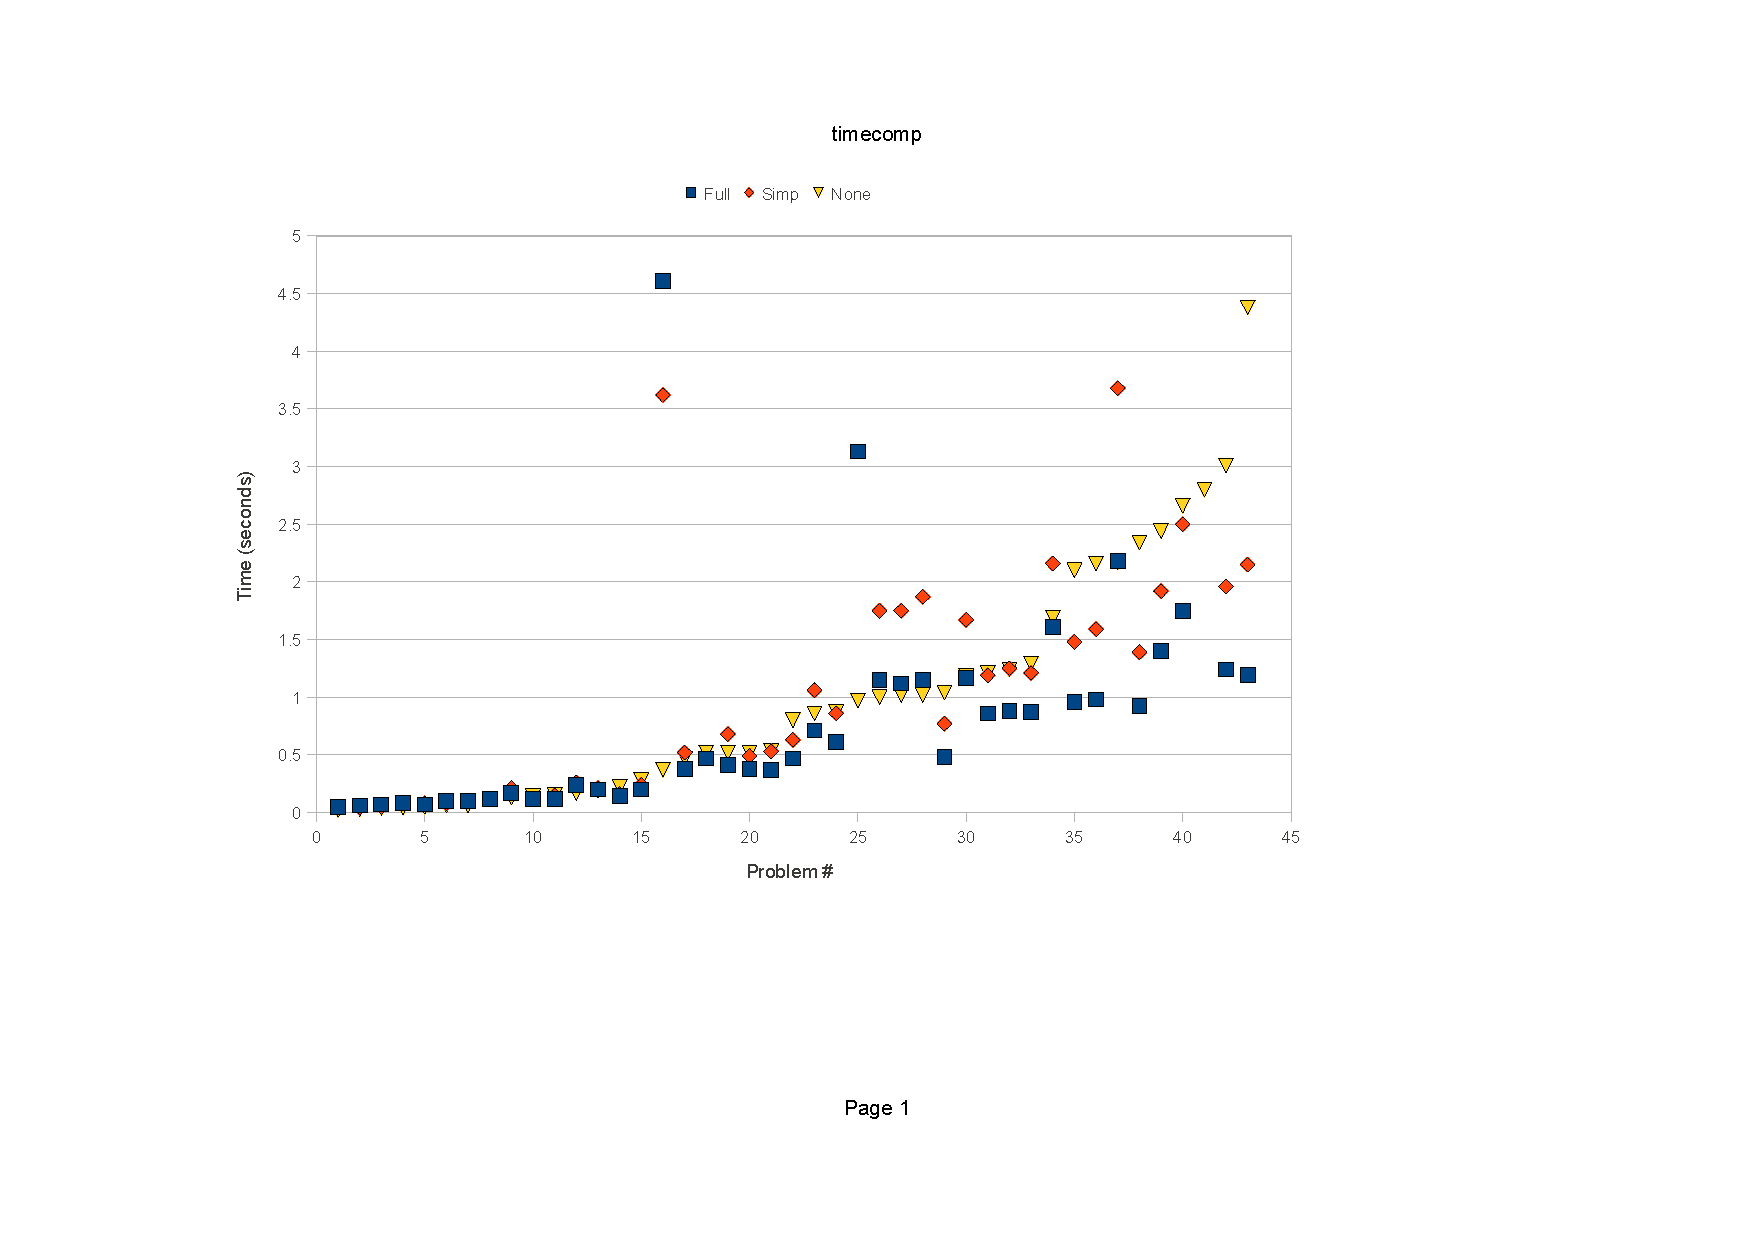
\includegraphics[scale=0.56,trim=3.7cm 5cm 0cm 3cm,clip]{suptime}
\end{frame}

\begin{frame}
  \frametitle{Runtimes under 5 seconds}
                  %Left Bot Right Top
  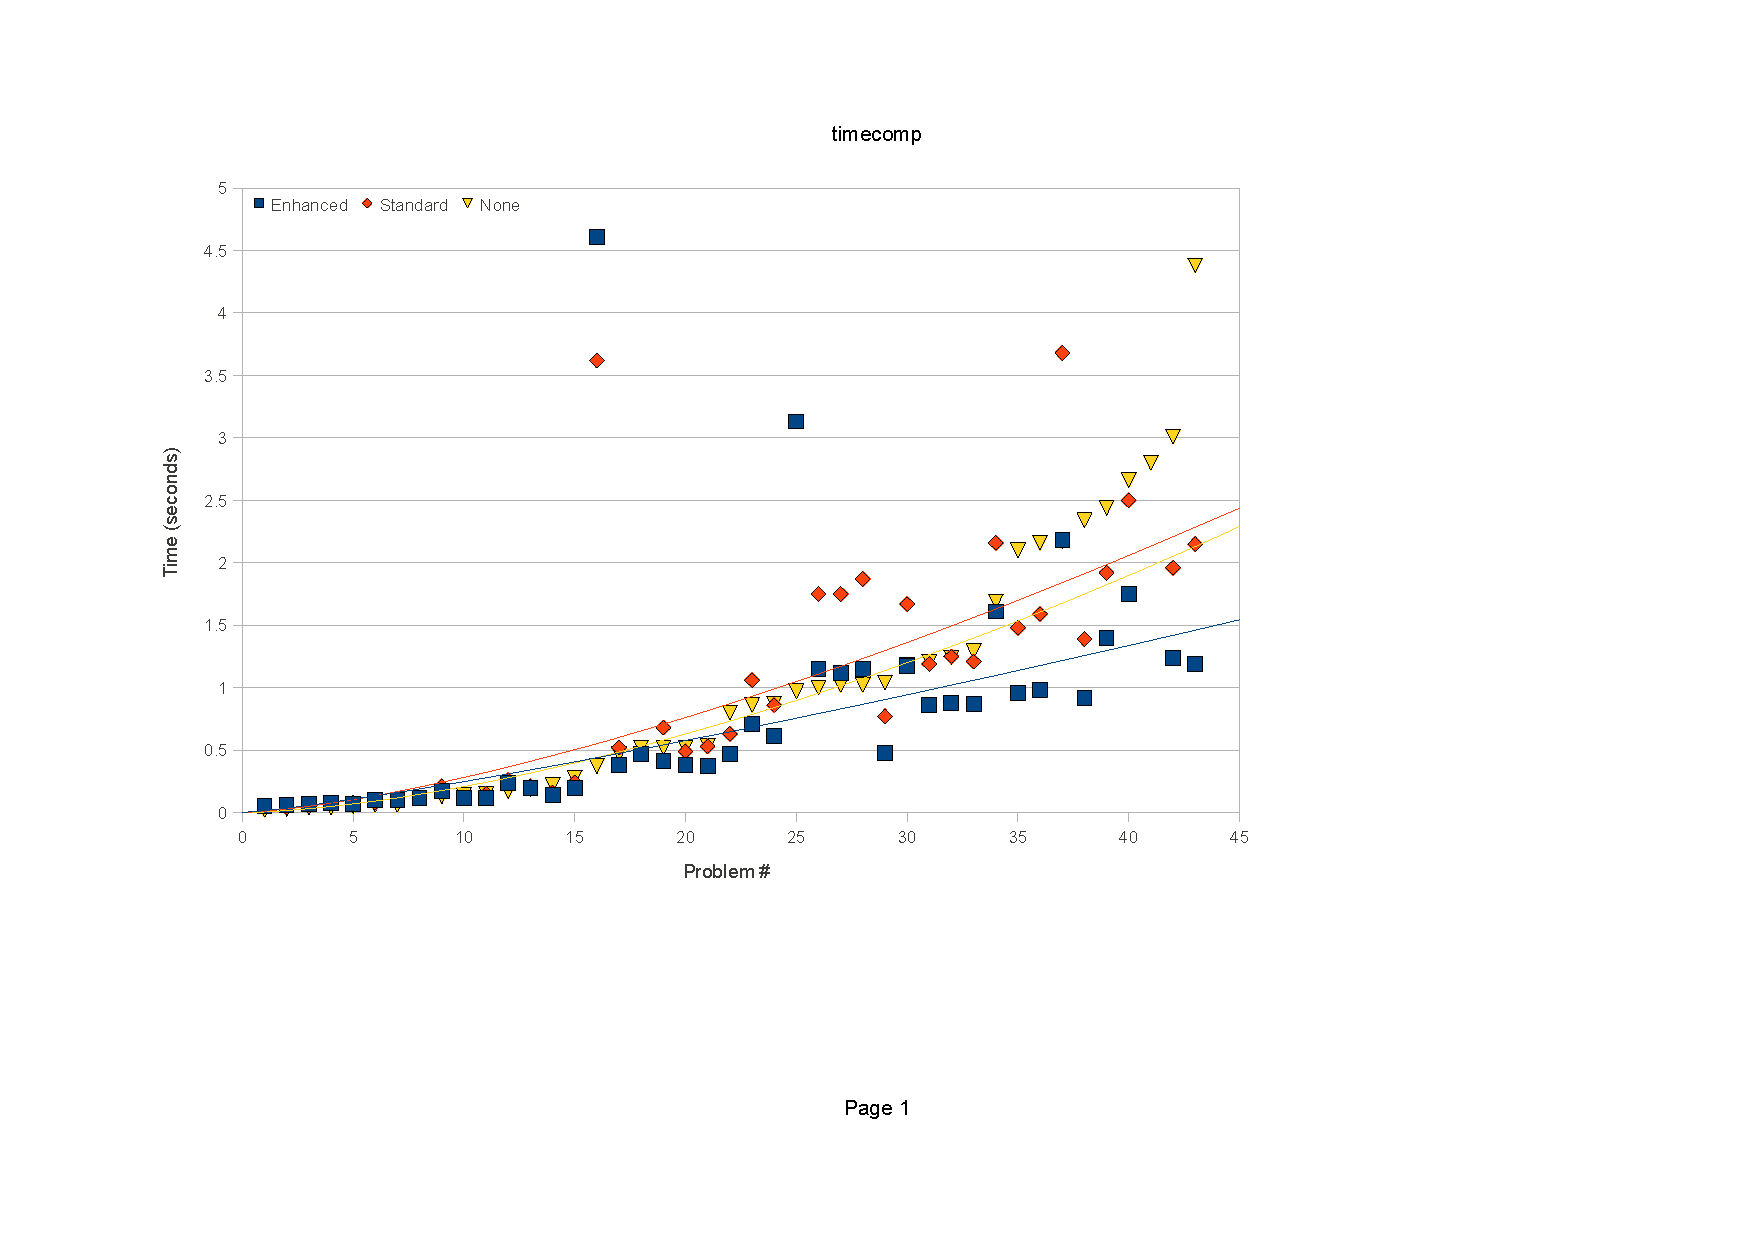
\includegraphics[scale=0.56,trim=2.45cm 5cm 0cm 3cm,clip]{suptimetrends}
\end{frame}


\begin{frame}
  \begin{itemize}
  \frametitle{Results Analysis}
  \item<1->[]
 \begin{table}[H]\scriptsize
  \caption{Superposition time for the 6 most extreme problem examples.}
\begin{tabular}{| l || r | r | r |}  \hline
Problem&Enhanced&Standard&Unmodified\\  \hline
DAT050=1.p&17.53& 31.54& 48.62\\
DAT039=1.p&13.2& 22.51& 130.77\\
DAT040=1.p&14.49& 21.29& 190.71\\
DAT038=1.p&12.53& 24.04& 294.86\\
DAT043=1.p&18.67& 26.08& \textbf{N/A} \\
DAT048=1.p&17.65& 35.77& \textbf{N/A}\\\hline
\end{tabular}\end{table}
  \item<2-> When taking number of inferences into account for DAT038=1.p we observe
  1.2 milliseconds per superposition for the full implementation versus 2.2 milliseconds
  per superposition for unindexed beagle.
  \end{itemize}
\end{frame}

%%%%%%%%%%%%%%%%%%%%%%%%%%
\subsection{Sample Position Comparisons}
%%%%%%%%%%%%%%%%%%%%%%%%%%
\begin{frame}
  \begin{itemize}
  \frametitle{Fingerprint Sampling Varieties}
  \item<1-> Reasoning. Cite shulz and FP/Speed balance
  \item<2-> Different position samples
  \end{itemize}
\end{frame}

\begin{frame}
  \frametitle{Fingerprint Sampling Varieties}
\begin{table}[H]\scriptsize
  \caption{Totalled inference counts and indexing statistics for various Fingerprint sampling sets.}
\begin{tabular}{| l || r | r | r || r | r | r |}  \cline{2-7}
\multicolumn{1}{ c }{} & \multicolumn{3}{ |c|| }{\textbf{Inference Counts}} & \multicolumn{3}{ c| }{\textbf{Indexing Results}} \\ \cline{1-7}
Sample Set&Sup&Demod&NegUnit&TotalFound&SupFP&SimpFP\\  \cline{1-7}
\textbf{FP3W}&162218&42402&2472&13913606&69429&1815992\\
\textbf{FP4M}&147798&35709&1963&13469779&26847&1851515\\
\textbf{FP6M}&144505&35326&1959&12601762&16406&1694731\\
\textbf{FP7}&159055&41005&2440&13011130&21281&1596575\\
\textbf{FP8X2}&159385&40876&2438&12819184&11229&1602033\\ \hline 
\end{tabular}\end{table}

\begin{table}[H]\scriptsize
  \caption{Totalled timing results for various Fingerprint sampling sets.}
\begin{tabular}{| l || r | r | r | r | r | r |}  \cline{2-7}
\multicolumn{1}{ c }{} & \multicolumn{6}{| c| }{\textbf{Time Spent (seconds)}} \\ \cline{1-7}
Sample Set&Indexing&Retrieving&Sup&Demod&NegUnit&Total\\  \cline{1-7}
\textbf{FP3W}&11.52&14.02&170.37&9.26&1.78&237.75\\
\textbf{FP4M}&13.09&14.12&164.95&9.51&1.82&230.68\\
\textbf{FP6M}&16.82&16.5&159.93&10.78&2.11&229.59\\
\textbf{FP7}&19.98&18.74&170.83&12.37&2.37&249.22\\
\textbf{FP8X2}&45.56&32.59&181.43&21.45&4.06&294.8\\ \hline 
\end{tabular}\end{table}
Note that for more relevant comparisons these results exclude PUZ037-1.p.
\end{frame}

%%%%%%%%%%%%%%%%%%%%%%%%%%%%%%%%%%%%%%%%%%%%%%%%%%%%%%%%%%%%%%%%%%%%%%%%%%%%%%%%
\section{Conclusion}
%%%%%%%%%%%%%%%%%%%%%%%%%%%%%%%%%%%%%%%%%%%%%%%%%%%%%%%%%%%%%%%%%%%%%%%%%%%%%%%%

\begin{frame}
  \begin{itemize}
  \frametitle{The Benefits of Indexing Beagle}
  \item<1-> The \HSWAC\ is a 
  \item<2-> 
  \end{itemize}
\end{frame}


\end{NoHyper}
\end{document}
